\section{Gestión del alcance}

\subsection{Entregables}
En este proyecto se busca brindar la posibilidad de mejorar la plataforma digital que cuenta la organización Animales sin hogar, añadiendo calidad a dicha plataforma y nuevas funcionalidades que permitan ayudar y potenciar al equipo que lleva las tareas del día a día en la organización.
Teniendo en cuenta las solicitudes que están detalladas, se puede hacer el siguiente sumario de entregables:


\prettyTable{|l|l|l|l|l|}{
    \textbf{Entregable} & \textbf{\mlcell{Criterio de \\aceptación}} & \textbf{\mlcell{Modalidad de \\aceptación}} & \textbf{\mlcell{Plazo de \\aprobación}} & \textbf{\mlcell{Responsable \\de aprobación}} \\ \hline
    
    
    \mlcell{ESRE de \\funcionladides \\existentes} & \mlcell{Cumple con detalle \\lo solicitado} & \mlcell{Correo \\electrónico} & \mlcell{2 días \\habiles} & \mlcell{Dirección de \\animales sin hogar} \\ \hline
    
    \mlcell{ESRE de \\nuevas \\funcionladides} & \mlcell{Cumple con detalle \\lo solicitado} & \mlcell{Correo \\electrónico} & \mlcell{2 días \\habiles} & \mlcell{Dirección de \\animales sin hogar} \\ \hline
    
    \mlcell{Ponderacion \\ de nuevas \\ funcionalidades} & \mlcell{Las prioridades \\ descriptas son \\acordes a la realidad} & \mlcell{Correo \\electrónico} & \mlcell{1 días \\habiles} & \mlcell{Dirección de \\animales sin hogar} \\ \hline
    
    \mlcell{Prototipo mejora de \\interfaz gráfica} & \mlcell{El 100\% de la interfaz\\ cumple al menos dos\\ heurísticas de Nielsen} & \mlcell{Correo electrónico} & \mlcell{3 días \\habiles} & \mlcell{Dirección de \\animales sin hogar} \\ \hline
    
    \mlcell{Prototipo bugs resueltos} & \mlcell{Todos los bugs reportados \\son resueltos.} & \mlcell{Correo \\electrónico} & \mlcell{3 días \\habiles} & \mlcell{Dirección de \\animales sin hogar} \\ \hline
    
    \mlcell{Prototipo con login} & \mlcell{El sistema implementa un \\correcto manejo de sesión} & \mlcell{Correo \\electrónico} & \mlcell{3 días \\habiles} & \mlcell{Dirección de \\animales sin hogar} \\ \hline
    
    \mlcell{Prototipo con login} & \mlcell{El sistema implementa un \\correcto manejo de sesión} & \mlcell{Correo \\electrónico} & \mlcell{3 días \\habiles} & \mlcell{Dirección de \\animales sin hogar} \\ \hline
    
    \mlcell{Prototipo con \\registro de animales} & \mlcell{El sistema permite \\ registrar animales} & \mlcell{Correo \\electrónico} & \mlcell{3 días \\habiles} & \mlcell{Dirección de \\animales sin hogar} \\ \hline
    
    \mlcell{Prototipo con \\registro de padrinos} & \mlcell{El sistema permite \\ registrar padrinos} & \mlcell{Correo \\electrónico} & \mlcell{3 días \\habiles} & \mlcell{Dirección de \\animales sin hogar} \\ \hline
    
    \mlcell{Casos de prueba \\registro de animales} & \mlcell{Cobertura de pruebas \\ unitarias 90\% y \\pruebas de equivalencia \\con casos borde} & \mlcell{Correo \\electrónico} & \mlcell{1 días \\habiles} & \mlcell{Gerente de proyecto} \\ \hline
    
    \mlcell{Casos de prueba \\registro de padrinos} & \mlcell{Cobertura de pruebas\\ unitarias 90\% y \\pruebas de equivalencia \\con casos borde} & \mlcell{Correo \\electrónico} & \mlcell{1 días \\habiles} & \mlcell{Gerente de proyecto} \\ \hline
        
    \mlcell{Mejora de \\pruebas unitarias} & \mlcell{Las pruebas unitarias tienen \\una cobertura del 90\%} & \mlcell{Correo \\electrónico} & \mlcell{1 días \\habiles} & \mlcell{Gerente de proyecto} \\ \hline
    
    \mlcell{Casos de prueba \\login} & \mlcell{Cobertura de pruebas\\ unitarias 90\% y \\pruebas de equivalencia \\con casos borde} & \mlcell{Correo \\electrónico} & \mlcell{1 días \\habiles} & \mlcell{Gerente de proyecto} \\ \hline
    
    \mlcell{Evidencia de \\pruebas realizadas} & \mlcell{El reporte de ejecución \\de pruebas evidencia \\el 100\% de las pruebas} & \mlcell{Correo \\electrónico} & \mlcell{1 días \\habiles} & \mlcell{Gerente de proyecto} \\ \hline
}


\subsection{Estructura de descomposición del trabajo}

Dado el anterior listado de entregables se puede modelar el EDT como muestra la figura \ref{fig:edt}, mas adelante en la sección de estimaciones listamos todas las actividades asociadas a cada uno de estos entregables.

\begin{figure}[H]
    \centering
    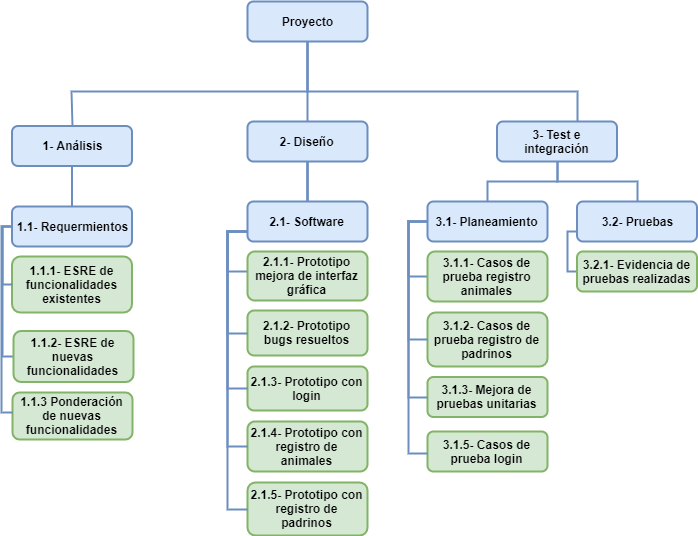
\includegraphics[scale=0.6]{Files/edtv4.png}
    \caption{Diagrama EDT}
    \label{fig:edt}
\end{figure}

